\subsection{Technologies, tools and frameworks}
\subsubsection{React}
React is a fast, declarative and efficient javascript library for creating web interfaces. It works around the concept of components. They are self-contained and composable blocks of code that encapsulates a part of user interface and its functionality. By putting together multiple small components it's possible to build complex user interfaces (UI). Components can be stateful or stateless.
The library provides a virtual-dom similar to the browsers document object model (DOM). They are both node trees that list elements together with attributes and content as objects and properties. Updating the dom is rather slow which is why the virtual-dom is useful for efficiency. It allows react to optimize DOM updates under the hood to only happen when it's necessary.
\subsubsection{Docker \& Containers}
Containers are self-contained pieces of code that can be run on any computer and operating system (OS). They contain the code and all of its necessary parts such as libraries, tools ,and frameworks. They are similar to virtual machines but the main difference is in efficiency and application size. Containers are more efficient and smaller because they run on the same underlying kernel as the operating system as opposed to virtual machines which runs an entirely different OS.

Docker is tool that allows creating, running and managing containers.
Docker

\begin{figure}[h!]
    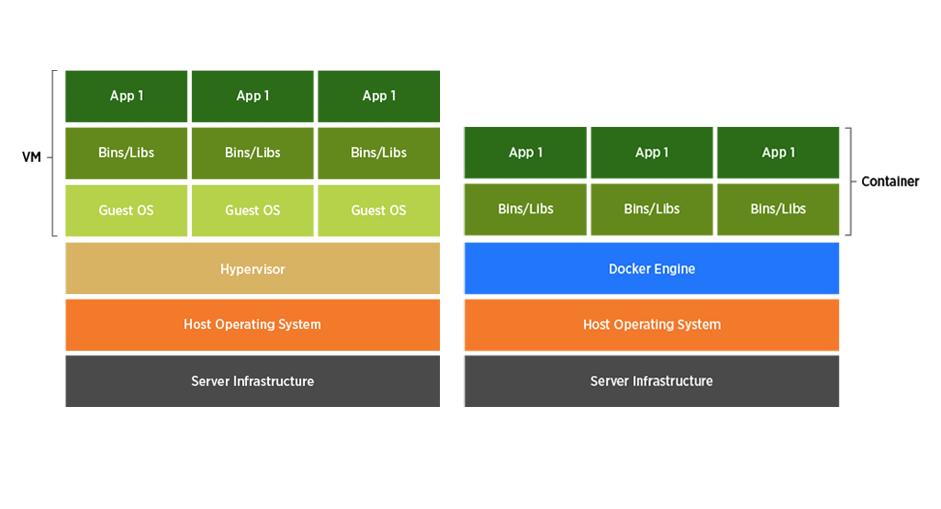
\includegraphics[scale=0.5]{containers-vs-vm-diagram}
    \caption{Containers and virtual-machine comparison diagram}
\end{figure}

\subsubsection{Kubernetes}
Kubernetes is a container orchestration platform created by Google and open-sourced in 2014. It allows automation of deployment, scaling, and management of containerized applications. It groups the containers that make up a multi micro-service application into logical units for easy discovery and management. It's built with scalability in mind 

Node 
Pod
Service
Gateway
Ingress

\subsubsection{Mongodb \& Mongoose}

\subsection{Micro-services}
Authentication

Gateway

User

Search

Engine

\begin{figure}[h!]
    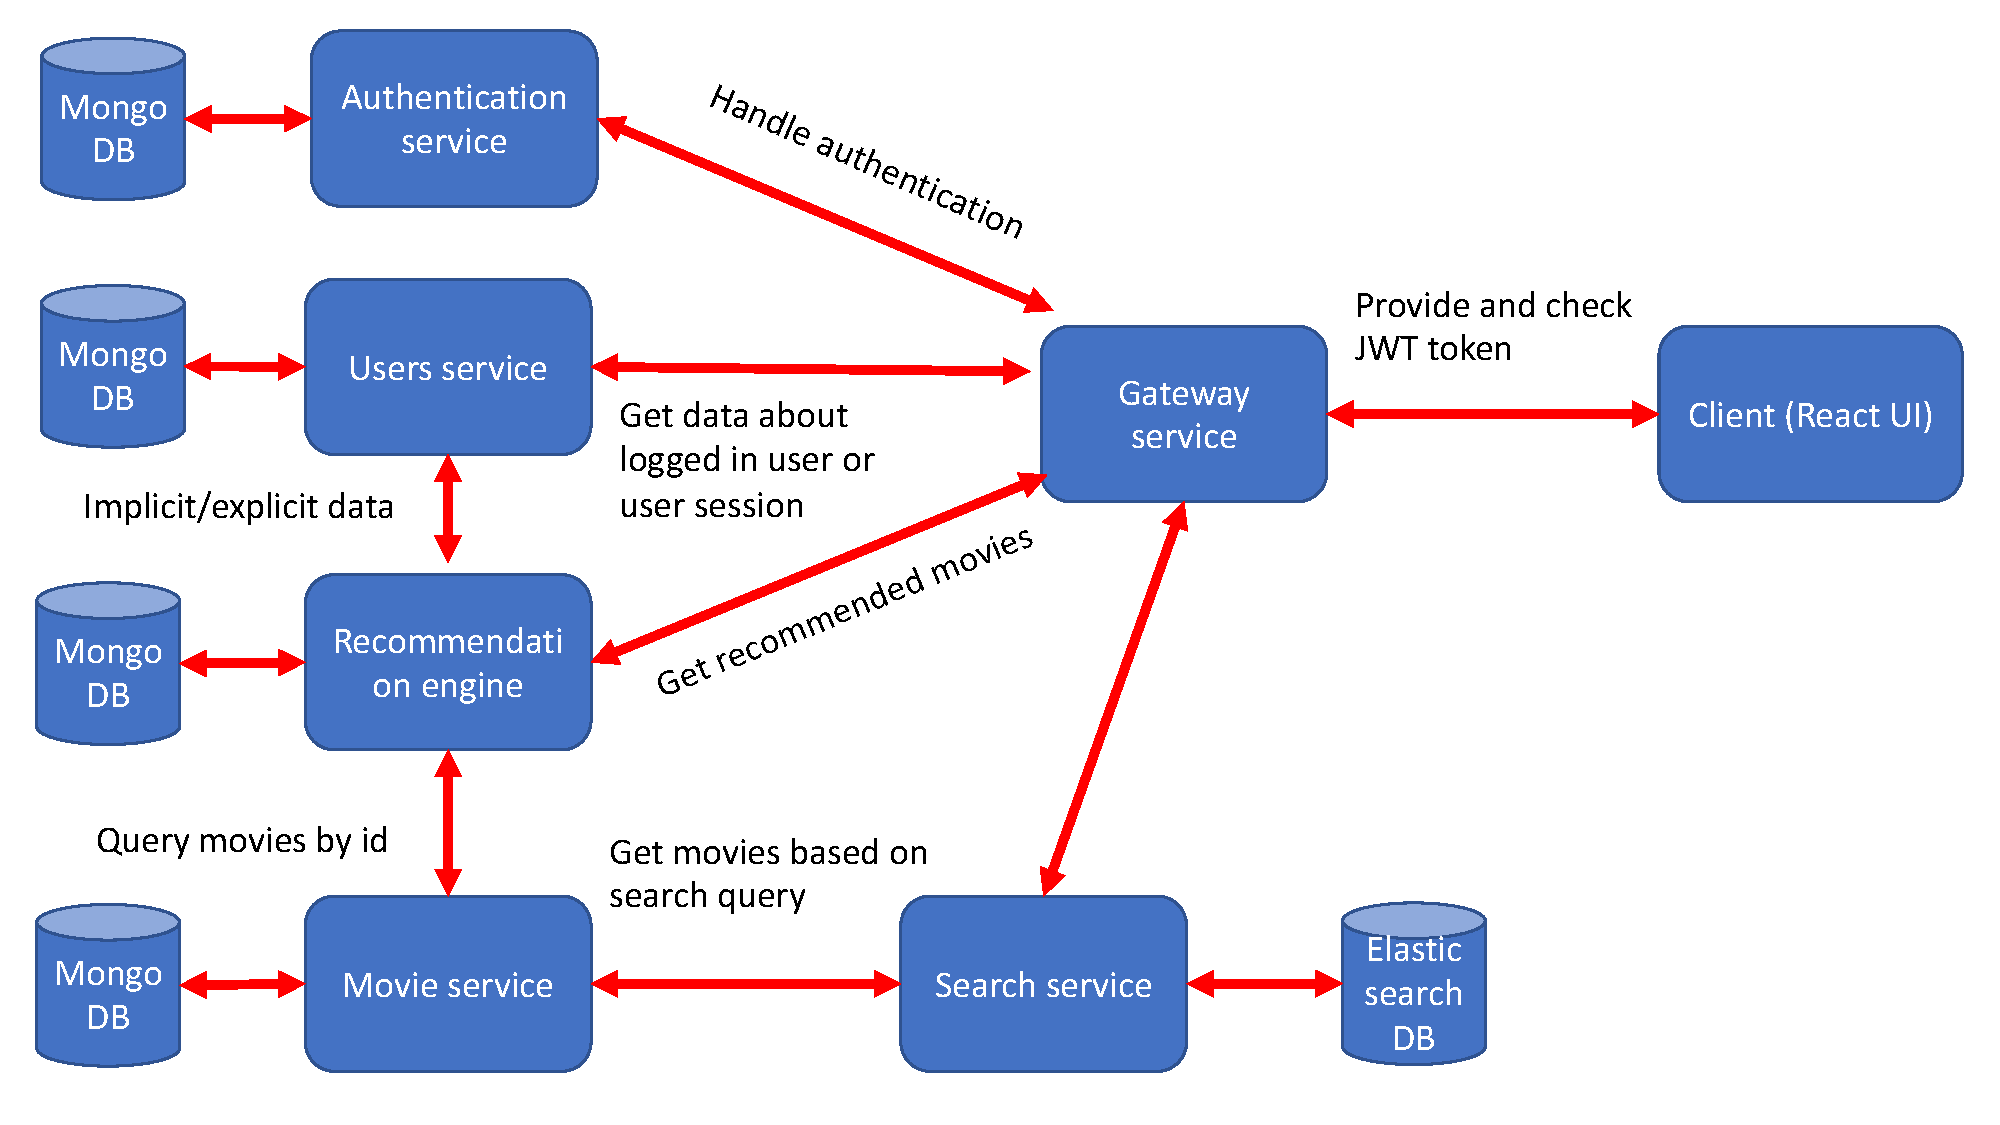
\includegraphics[scale=0.4]{architecture_diagram}
    \caption{Architecture diagram}
\end{figure}

\begin{figure}[h!]
    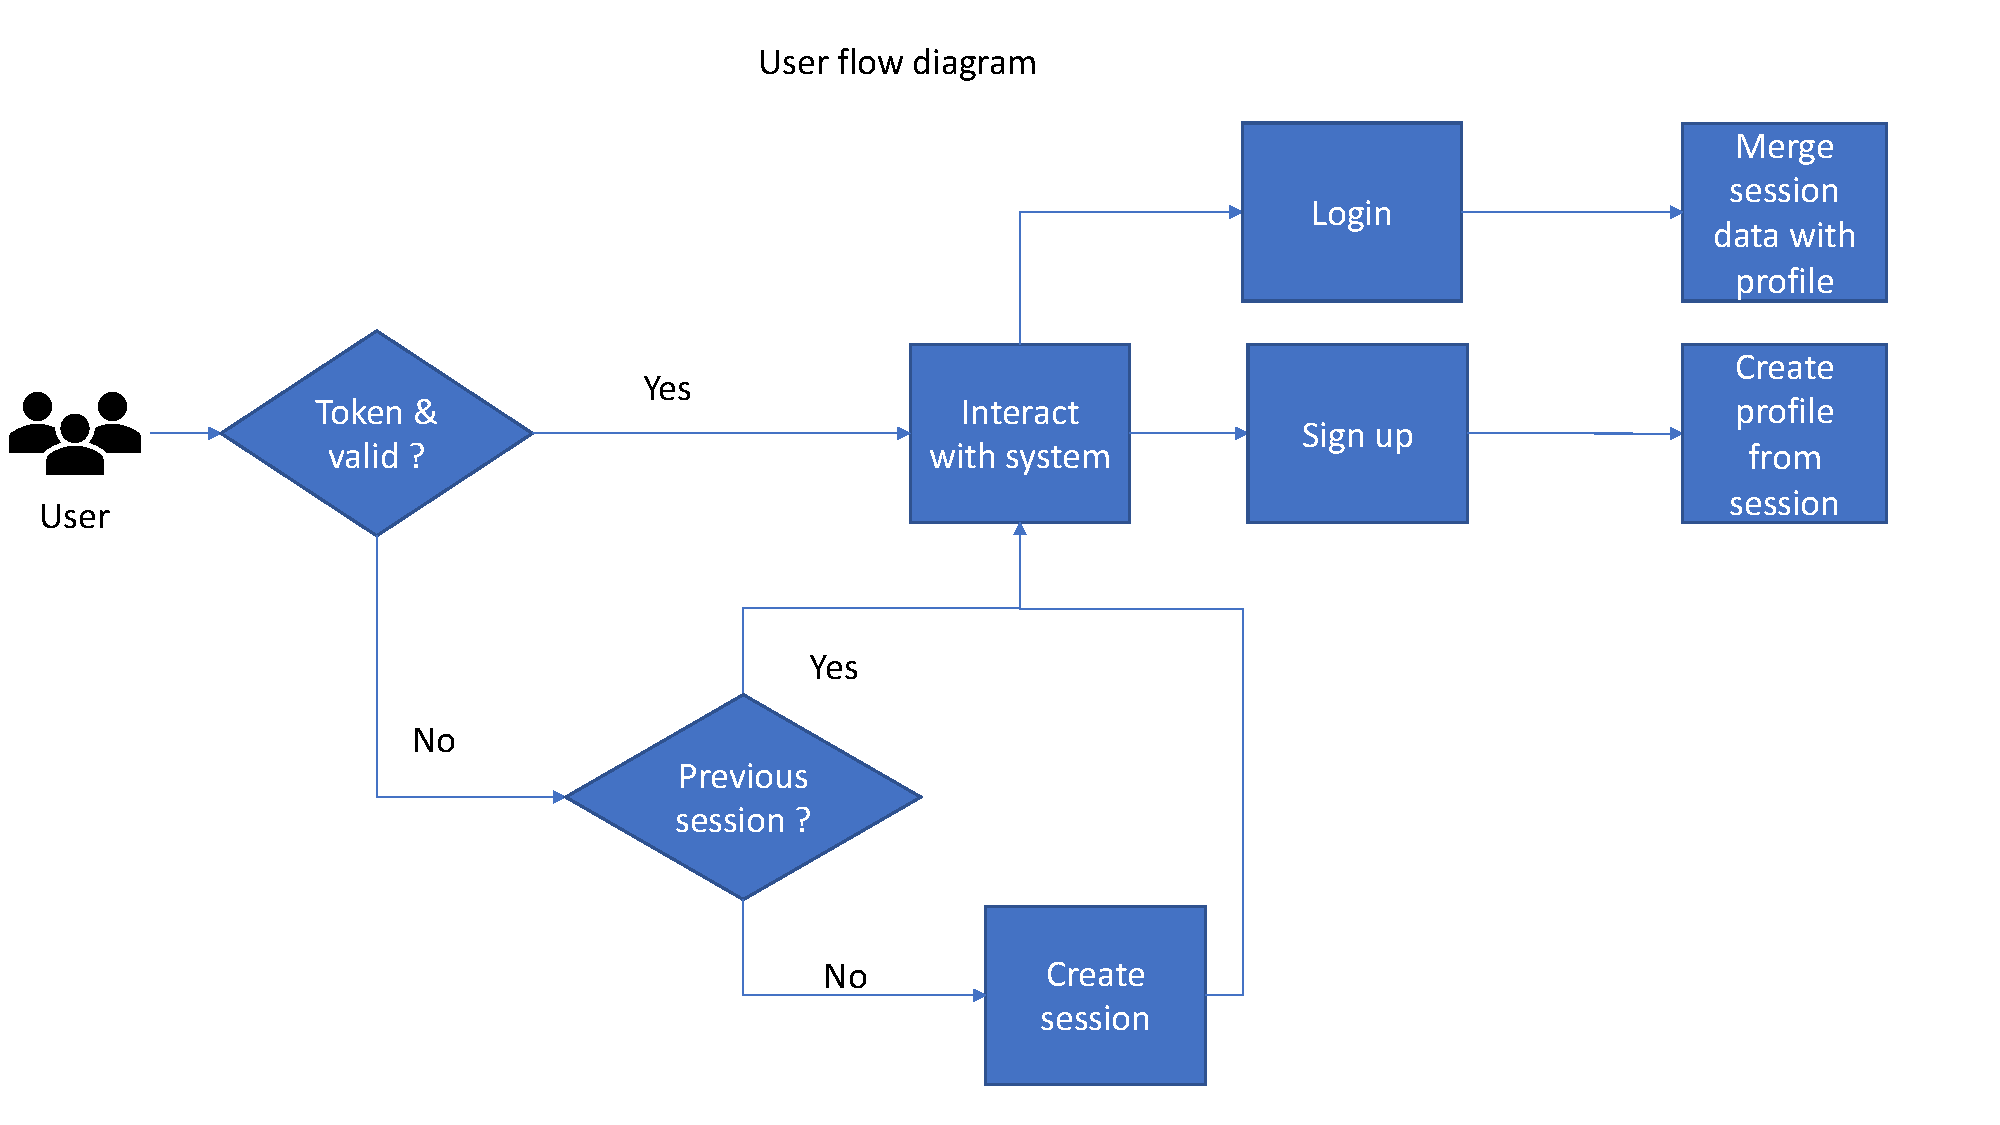
\includegraphics[scale=0.4]{user_flow_diagram}
    \caption{User flow diagram}
\end{figure}

% \subsection{Database}
\subsection{Web application}